\section{Modeling expert speakers and uncertain listeners}\label{sec:model}

Simple communication games provide the basis for our
model. Intuitively, these models involve a speaker trying to convey
some information to the listener with language that potentially
under-determines that information.  The basic structure traces to the
signaling systems of \cite{Lewis69}:

\begin{definition}[Communication games]\label{def:struc} 
  A communication game is a structure $\Cgame$:
  \begin{enumerate}\setlength{\itemsep}{0pt}
  \item $\States$ is a set of states (worlds, referents, propositions, etc.).
  \item $\Messages$ is a set of messages.
  \item $\Lex: \Messages \mapsto \wp(\States)$ is a lexicon.
  \item $\Prior : \States \mapsto [0,1]$ is a prior probability
    distribution over states.   
  \item $\Costs : \Messages \mapsto \Reals$ is a cost function on messages.
  \end{enumerate}
\end{definition}

In a communication game, the speaker observes a state $\state$ and
chooses a message $\msg$ based on $\state$ and the message costs
$\Costs$. The listener chooses a state $\state'$ based on $\msg$ and
her prior expectations $\Prior$ about the state.  We assume throughout
that the speaker will choose a message that has maximum probability
given the state, and that the hearer will choose a state that has
maximum probability given the speaker's message.  This amounts to the
assumption that the speaker and hearer would like to communicate,
which might or might not be tied up with their real-world goals
\cite{Franke-etal:2009,Asher:Lascarides:2013}

Production and interpretation can be modeled as a recursive process in
which the speaker and listener reason about each other reasoning about
each other.  Suppose we begin with a truth-conditional listener
$\GenericListener$: given message $\msg$, $\GenericListener$ guesses a
state $\state \in \Lex(\msg)$ based only on the prior.  The speaker
$\GenericSpeaker$ can model this truth-conditional listener in
production, anticipating her inferences and trying to respond in a way
that maximizes the chances of successful communication.  What's more,
$\GenericListener$ can plan for this kind of sophisticated speaker and
make her inferences accordingly.  And so forth. The process can
proceed until the system stabilizes or until the participants reach
the limits of their rationality, mental energy, or commitment to the
cause
\cite{CamererHo:2004,Franke:2008,Franke09DISS,Jaeger:2007,Jaeger:2011}.
The basic dynamics of this recursive process have been shown to derive
many kinds of pragmatic enrichment, that is, inferences that go beyond
the content literally encoded in the language used.

Fleshing out the above intuitive ideas, we begin with the most basic
listener, $\listenerZero$, which simply uses the truth-conditions of
the message $\msg$ and the prior over states to estimate a conditional
probability distribution over states:

\begin{definition}[$\listenerZero$]\label{def:l0}
  \[
  \listenerZero(\state \given \msg, \Lex)
  \propto
  \frac{\mathbb{I}(\state \in \Lex(\msg))}{|\Lex(\msg)|}
  \Prior(\state)
  \]
\end{definition}

The most basic speaker $\speakerOne$ reasons about $\listenerZero$,
taking message costs into account. In other words, this agent plans
its utterances with $\listenerZero$'s expected behavior in mind,
making it a pragmatic agent in a limited sense:

\mynote{Once the definitions are finalized, we can explicate the parameters.}

\mynote{Could we get by without $\lambda$ and $\gamma$ in this paper, just to reduce the number of parameters?}

\begin{definition}[$\speakerOne$]\label{def:s1}  
  \[
  \speakerOne(\msg \given \state, \Lex) 
  \propto
  \exp
  \left(
    \lambda
    (
      \log
      (\listenerZero(\state \given \msg, \Lex))
      - \gamma\Costs(\msg)
     )
  \right)
  \]
\end{definition}

The $\listenerOne$ listener responds to $\speakerOne$ in the sense
that it reasons about that agent and the priors; the definition is
parallel to the one for $\listenerZero$ except that the starting point
is the pragmatic distribution $\speakerOne$ rather than the truth
conditions given directly by $\Lex$:

\begin{definition}[$\listenerOne$]\label{def:l1}
  \[
  \listenerOne(\state \given \msg, \Lex) 
  \propto 
  \speakerOne(\msg \given \state, \Lex)\Prior(\state)
  \]
\end{definition}

\mynote{Could pause here to illustrate a scalar implicature of some kind using a communication game}

The agents $\speakerOne$ and $\listenerOne$ could iteratively respond
to each other until their communication systems stabilized. Such
interactions are able to model many of the core phenomena studied
under the heading of Gricean pragmatics.  However, the model falls
short of generating the full range of such inferences.  One way to
address this is to introduce uncertainty about the lexicon $\Lex$ and
allow it to interact with the built-in uncertainty of the states and
messages.

The above are all lexicon-specific in the sense that the basic
semantic interpretation function $\Lex$ remains fixed throughout all
the calculations.  However, the members a speech community never have
complete knowledge of the precise conventions that govern that
community, and those norms are constantly evolving anyway. As a
result, speakers and listeners are generally willing to entertain a
wide range of different lexicons, to assume that others will entertain
such lexicons, and so forth, and this indeterminacy has itself been
argued to stimulate a range of pragmatic inferences
\cite{Bergen:Goodman:Levy:2012,Bergen:Goodman:2014}. Thus, we now
extend the basic model with agents that manage linguistic uncertainty
as well as factual uncertainty.

The agent $\ListenerOne$ is the first in the hierarchy to reason in
terms of $\Lex$; this listener is identical to the ``social anxiety''
listener of \cite{Smith:Goodman:Frank:2013}. It forms a posterior over
lexica and marginalizes over this posterior to form beliefs about
communicated meaning:

\begin{definition}[$\ListenerOne$]\label{def:l1}
  \begin{align*}
  \ListenerOne(\state, \Lex \given \msg) 
  &= 
  \sum_{\Lex} \listenerOne(\state \given \msg, \Lex) \ListenerOne(\Lex \given \msg) 
  \\
  \ListenerOne(\Lex \given \msg) &\propto \Prior(\Lex) \sum_{\state\in\States} \speakerOne(\msg \given \state)\Prior(\state)
  \end{align*}
\end{definition}

\mynote{Could pause here to illustrate a manner implicature of some kind}

At this point, one might consider extending this lexical uncertainty
to the listener, as is done in \cite{Smith:Goodman:Frank:2013}.
However, in situations involving (organized or impromptu) language
pedagogy, the speaker does not have lexical uncertainty in the
relevant sense.  Rather, she knows the (relevant aspects of) the
lexicon $\LexStar$ that she intends to use. Furthermore, she places
value on the listener $\ListenerOne$'s correct apprehension of
$\LexStar$. This socially confident, pedagogically-minded speaker is
defined as follows:

\begin{definition}[$\ListenerK$]\label{def:l1}
  \begin{align*}
  \ListenerK(\state, \Lex \given \msg) 
  &= 
  \sum_{\Lex} \listenerOne(\state \given \msg, \Lex) \ListenerK(\Lex \given \msg) 
  \\
  \ListenerK(\Lex \given \msg) &\propto \Prior(\Lex) \sum_{\state\in\States} \SpeakerK(\msg \given \state, \Lex = \LexStar)\Prior(\state)
  \end{align*}
\end{definition}

\begin{definition}[$\SpeakerK$]\label{def:l1}
  $\SpeakerK(\msg \given \state, \LexStar) \propto$
\end{definition}

\Figref{fig:model} summarizes the relationship between the above
agents, highlighting the point at which lexical uncertainty is
introduced. In our model, all agents $\SpeakerK[2]$ and higher are
expert speakers in the sense that they presume a fixed lexicon
$\LexStar$ about which they seek to instruct the listener via language
use.

\begin{figure}[htp]
  \centering
  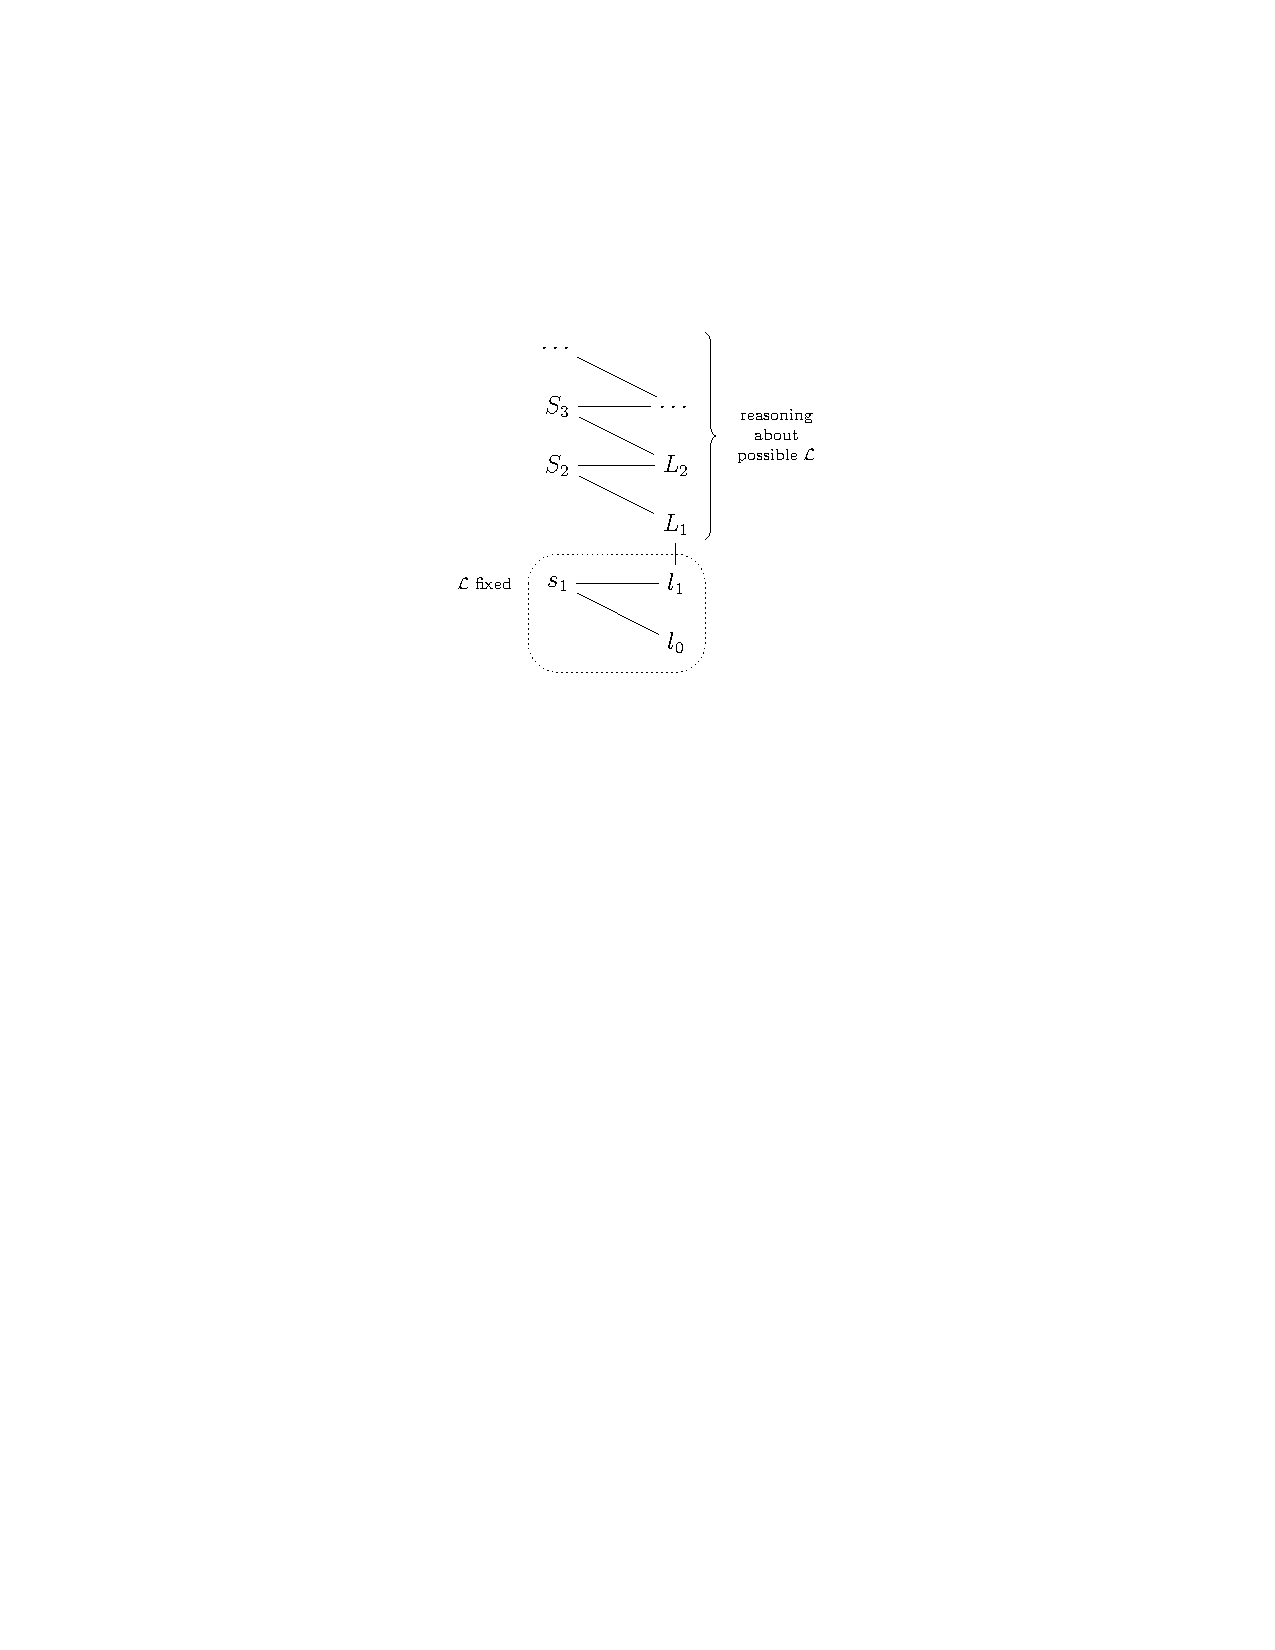
\includegraphics[scale=1]{images/model}
  \caption{Pictoral representation of the recursive reasoning process.}
  \label{fig:model}
\end{figure}

%%% Local Variables: 
%%% mode: latex
%%% TeX-master: "definitional_disjunction"
%%% End: 


